\subsection{UC5: Gestione degli alert}
\hypertarget{UC5}{}
\begin{figure} [H]
	\centering
	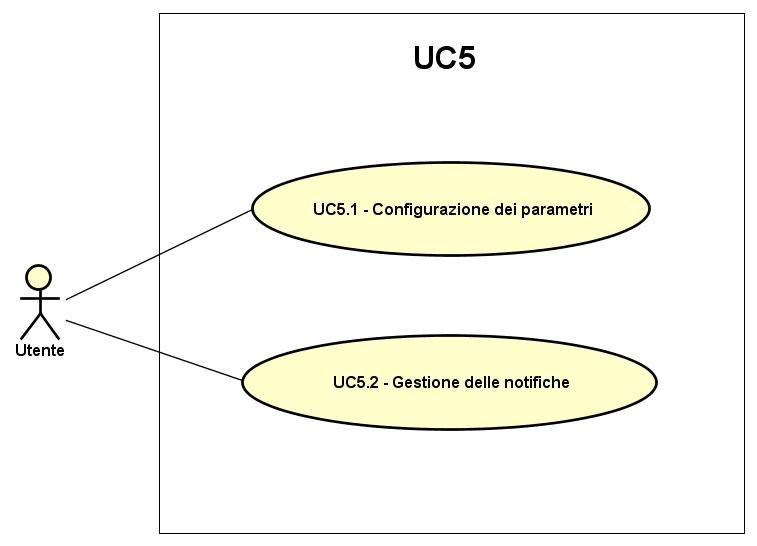
\includegraphics[scale=0.45]{Img/UC5}
	\caption{UC5 - Gestione degli alert}\label{}
\end{figure}
\begin{itemize}
	\item \textbf{Attori}: Utente;
	\item \textbf{Descrizione}: l'attore configura le opzioni relative ad alert personalizzati;
	\item \textbf{Precondizione}: il plug-in deve leggere un flusso di dati;
	\item \textbf{Flusso principale degli eventi}:
	\begin{itemize}
		\item Configurazione dei parametri (UC5.1);
		\item Gestione delle notifiche (UC5.2).
	\end{itemize}
	\item \textbf{Postcondizione}: gli alert e le notifiche di attivazione sono stati configurati.
\end{itemize}

\subsection{UC5.1: Configurazione dei parametri}
\hypertarget{UC5.1}{}
\begin{figure} [H]
	\centering
	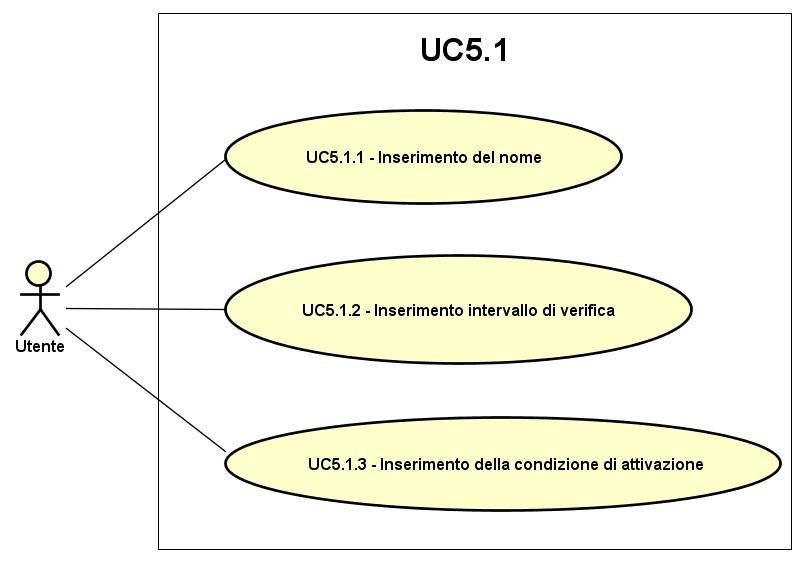
\includegraphics[scale=0.45]{Img/UC5-1}
	\caption{UC5.1 - Configurazione dei parametri}\label{}
\end{figure}
\begin{itemize}
	\item \textbf{Attori}: Utente;
	\item \textbf{Descrizione}: l'attore configura i parametri che definiscono un alert;
	\item \textbf{Precondizione}: il sistema permette la configurazione dei parametri di un alert;
	\item \textbf{Flusso principale degli eventi}:
	\begin{itemize}
		\item Inserimento del nome (UC5.1.1);
		\item Inserimento intervallo di notifica (UC5.1.2);
		\item Inserimento della condizione di attivazione (UC5.1.3).
	\end{itemize}
	\item \textbf{Postcondizione}: l'alert è stato configurato.
\end{itemize}

\subsection{UC5.1.1: Inserimento del nome}
\hypertarget{UC5.1.1}{}
\begin{itemize}
	\item \textbf{Attori}: Utente;
	\item \textbf{Descrizione}: l'attore inserisce il nome dell'alert;
	\item \textbf{Precondizione}: il sistema permette l'inserimento del nome di un alert;
	\item \textbf{Postcondizione}: il nome dell'alert è stato inserito.
\end{itemize}

\subsection{UC5.1.2: Inserimento intervallo di verifica}
\hypertarget{UC5.1.2}{}
\begin{itemize}
	\item \textbf{Attori}: Utente;
	\item \textbf{Descrizione}: l'attore inserisce l'intervallo di verifica ed una eventuale durata minima della condizione di attivazione per notificare l'alert;
	\item \textbf{Precondizione}: il sistema permetta l'inserimento dell'intervallo di verifica di un alert;
	\item \textbf{Postcondizione}: l'intervallo di verifica dell'alert è stato inserito.
\end{itemize}

\subsection{UC5.1.3: Inserimento della condizione di attivazione}
\hypertarget{UC5.1.3}{}
\begin{itemize}
	\item \textbf{Attori}: Utente;
	\item \textbf{Descrizione}: l'attore inserisce la condizione necessaria per l'attivazione dell'alert;
	\item \textbf{Precondizione}: il sistema permette l'inserimento di una condizione di attivazione di un alert;
	\item \textbf{Postcondizione}: la condizione di attivazione dell'alert è stata inserita.
\end{itemize}

\subsection{UC5.2: Gestione delle notifiche}
\hypertarget{UC5.2}{}
\begin{itemize}
	\item \textbf{Attori}: Utente;
	\item \textbf{Descrizione}: l'attore seleziona il modo in cui viene notificata l'attivazione di un alert;
	\item \textbf{Precondizione}: il sistema permette di notificare l'attivazione di un alert;
	\item \textbf{Postcondizione}: il modo in cui viene notificata l'attivazione di un alert è stato selezionato.
\end{itemize}
